\documentclass{subfiles}
\begin{document}
    \begin{figure}[!hb]
        \centering
        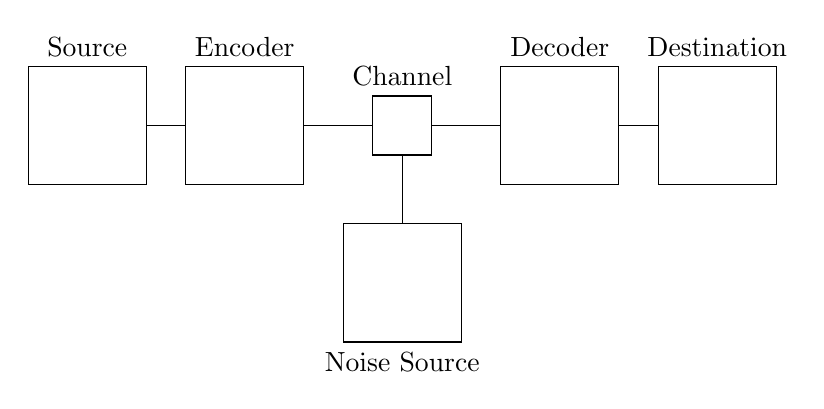
\begin{tikzpicture}[
            square/.style={draw, rectangle, minimum size=1.5cm, inner sep=0pt},
            ch/.style={draw, rectangle, minimum size=0.75cm, inner sep=0pt}
        ]

        \node [square, label=above:{Source}] (IS) at (0, 0) {};
        \node [square, label=above:{Encoder}] (En) at (2, 0) {};
        \node [ch, label=above:{Channel}] (Ch) at (4, 0) {};
        \node [square, label=above:{Decoder}] (De) at (6, 0) {};
        \node [square, label=above:{Destination}] (Re) at (8, 0) {};
        \node [square, label=below:{Noise Source}] (No) at (4, -2) {};

        \draw (IS) -- (En) -- (Ch) -- (No)
            (Ch) -- (De) -- (Re);


        \end{tikzpicture}
        \caption{Diagram of a general communication system.}
        \label{Fig:1}
    \end{figure}
\end{document}

